% ---------------------------------------------------------------------------
% RECOMB 2027 submission: 10-page main text.
%
% RECOMB allows 10 Letter pages at 10pt minimum with 1-inch margins,
% bibliography excluded, plus a separate title page and an appendix of
% unlimited length (appendix.tex here). The full 20-page treatment stays in
% main.tex and on arXiv.
%
% Build:  pdflatex recomb10 && bibtex recomb10 && pdflatex recomb10 x2
% ---------------------------------------------------------------------------
\documentclass[10pt]{article}

\usepackage[utf8]{inputenc}
\usepackage[T1]{fontenc}
\usepackage[margin=1in]{geometry}
\usepackage{graphicx}
\usepackage{booktabs}
\usepackage{amsmath,amssymb}
\usepackage[expansion=false]{microtype}
\usepackage[labelfont=bf,font=small]{caption}
\usepackage[numbers,sort&compress]{natbib}
\usepackage[hidelinks]{hyperref}

\graphicspath{{../figures/}}
\renewcommand{\bibname}{References}

\title{\textbf{Factor-combination discovery is stochastic threshold group
testing: a counterfactual replay of the 2006 reprogramming screen}}

\author{Mashal Saleh Alkhalifah\thanks{Institute of Smart Cities, King
Abdulaziz City for Science and Technology (KACST), Riyadh, Saudi Arabia.
Correspondence: \texttt{mkhalifah@kacst.gov.sa}}}

\date{\today}

\begin{document}

% --- separate title page, permitted by the CFP and excluded from the limit
\maketitle
\thispagestyle{empty}
\begin{abstract}
\noindent
Finding the few transcription factors that drive a cell-fate conversion is
expensive: every query is a wet-lab assay, and the 2006 screen for the
reprogramming factors consumed a documented 61 under a fixed leave-one-out
protocol. We show that this class of screen is an instance of \emph{stochastic
threshold group testing}, and replay it on an oracle calibrated to published
assay figures. Five results follow. (1) Information-gain design recovers the
hidden recipe in a median of 10 experiments against 61, cheaper in 300 of 300
paired replicates; the same inference with random pools needs 44, locating the
gain in experiment selection, not inference. (2) An apparent scaling limit, a
classical search overtaking the designer at 48 candidates, is a property of
the proposals rather than the method: changing only which pools may be scored
drops the growth exponent from $n^{1.6}$ to $n^{0.43}$ at 100\% recovery,
where the classical search falls to 83\%. (3) Fixing the recipe cardinality
fails \emph{symmetrically and silently}, at 0.999 confidence whether the true
recipe is smaller or larger; making size latent removes this for one extra
experiment. (4) Audited against two measured perturbation datasets, the
assumed gap response of 0.10 should be 0.77; re-run on that structure the
designer as calibrated recovers 2.5\% of recipes, at mean posterior confidence
0.991 on its failures. (5) That precondition is removable: making the gap
response latent recovers 99.3\%, at 0.4 experiments above an oracle told its
value, and beats a five-experiment calibration pilot on cost and accuracy. The
replay validates the procedure, not the oracle, which was calibrated from the
screen replayed; only (4) tests it against independent data. Results 3--5 are
one finding: every assay parameter such a designer fixes is a silent failure
awaiting a system that disagrees, and the remedy is to make it latent rather
than calibrate it better.

\medskip
\noindent\textbf{Code, per-run results and the full statistical report:}\\
\url{https://github.com/mashal-alkhalifah/yamanaka-replay}
\end{abstract}
\newpage
\setcounter{page}{1}

% ===========================================================================
\section{Introduction}

A cell-fate conversion driven by defined factors is, computationally, a
subset-identification problem: of $n$ candidates an unknown subset $R$ of size
$k$ is sufficient, and the task is to find $R$. What makes it hard is not the
size of the space but the price of a query. Each query is a transduction
experiment with a biological readout, so budgets are counted in tens.

The canonical instance is the screen of \citet{takahashi2006}, extended to
human cells the following year \citep{takahashi2007}. Twenty-four candidates
were drawn from the literature; the readout was the number of drug-resistant
colonies surviving Fbx15/G418 selection; and the search followed a protocol
fixed in advance --- each factor alone, the full pool, leave-one-out from the
pool, then leave-one-out from the survivors --- consuming $2n + 13 = 61$
experiments at $n = 24$ regardless of what the data said.

Adaptive experimental design \citep{lindley1956, chaloner1995, rainforth2024}
should improve on a fixed protocol, and in perturbation biology several groups
have shown that it does \citep{zhang2023, tosh2025}. What has not been
established is the counterfactual for a specific documented discovery: not
predictive accuracy over an adaptively collected dataset, but the number of
wet-lab experiments needed to reach a known answer under the assay actually
used. The 2006 screen is a good vehicle precisely because its experiment count
is in the public record.

Our second contribution is a reclassification. The colony assay is not generic
combinatorial search: a pool produces colonies efficiently only when it
contains all of $R$, weakly when it contains all but one, and not at all
otherwise. In group-testing language \citep{dorfman1943, aldridge2019} a test
is negative at or below a lower threshold $l$, positive at or above an upper
threshold $u$, and stochastic in the gap $g = u - l - 1$. This is threshold
group testing \citep{damaschke2006} in its stochastic form \citep{chan2013},
with $u = k$, $l = k-2$ and $g = 1$. The reclassification is load-bearing: it
supplies a yardstick for the achievable test count, $O(g^2 d \log n)$, and
classical algorithms as baselines, and both change the conclusions one would
otherwise draw.

The third contribution is what the paper spends most of its space on. An
adaptive designer carries a model of the assay, and that model has parameters
its author must set. We show, three times over with three different
parameters, that fixing such a parameter produces not degraded performance but
\emph{confident error}: the search stops on its own criterion, inside budget,
and returns a wrong answer with a posterior above 0.99. Worse, efficiency
aggravates it --- a protocol that runs 61 experiments gives 61 chances to
notice the model is wrong, while a designer that runs 9 gives nine.

\paragraph{Related work.}
\emph{Group testing} supplies the problem class and its bounds
\citep{dorfman1943, aldridge2019}; the matching variant is threshold group
testing \citep{damaschke2006, chan2013}, whose designs continue to improve
\citep{bui2024}. Those designs are parameterised by a \emph{known} threshold
$u$, while here $u = |R|$ is exactly what the experimenter does not know.
Group testing is also being applied to biology now \citep{talamanca2026}, but
in its disjunctive form --- a pool is positive if it contains any positive
item --- whereas a reprogramming pool is positive only if it contains
\emph{all} of the recipe. \emph{Bayesian experimental design} supplies the
criterion \citep{lindley1956, chaloner1995, rainforth2024} and has been used to
choose genetic interventions \citep{zhang2023} and combination drug screens
\citep{tosh2025}; recent work amortises an acquisition policy over historical
CRISPR screens \citep{edwards2026} or selects gene pairs with a predictive
model in the loop \citep{qin2025}. These are evaluated on hit recovery or
predictive accuracy at a fixed budget fraction, not against a documented
experiment count. \emph{Prediction rather than design} ranks reprogramming
factors from expression and network data \citep{rackham2016}, scores
transcription-factor combinations from single-cell multiomics
\citep{tfcomb2025}, and predicts unseen multi-gene perturbation outcomes
\citep{roohani2022}; these produce a ranking to test, not a sequence of
experiments. \emph{Measured combinatorial perturbation data}
\citep{norman2019, joung2023, replogle2022, peidli2024} is what we audit the
assay model against in Section~\ref{sec:real}.

% ===========================================================================
\section{Methods}
\label{sec:methods}

\paragraph{Oracle.} The assay returns a Poisson count with rate
$\lambda(S) = B\, f(|S \cap R|)\, e^{-\delta \max(0,\,|S|-k)}$, where $f(k)=1$,
$f(k-1)=\rho$ and $f(j)=0$ for $j<k-1$. Constants are fitted to the figures
reported in \citet{takahashi2006}: $B = 45$, $\delta = 0.0357$ so that a
24-factor pool yields about 22 colonies, and $\rho = 0.10$ from the partial
colony formation reported for three-of-four pools. The pool-size penalty is
why the paper's 10-factor subset outperformed the full 24.

\paragraph{Inference.} The hypothesis space is every $k$-subset of the $n$
candidates, $\binom{24}{4} = 10{,}626$ at the historical size, carried as an
exact posterior. The count distribution depends on a hypothesis only through
$|S \cap h|$, so both the likelihood and the expected information gain collapse
to a mixture over $k+1$ overlap classes however many hypotheses remain alive:
choosing an experiment costs the same whether the posterior spans ten
hypotheses or ten thousand. We select the pool maximising mutual information
between the recipe and the outcome, and stop when one hypothesis exceeds 0.95.

\paragraph{Latent structure.} Recipe size becomes latent by indexing the
collapse with $|h|$ as well: hypotheses are all subsets of size 3--6
($189{,}750$), classes are the 22 reachable pairs $(|h|, |S \cap h|)$. The gap
response becomes latent the same way, indexing by a discretised assay model
$m$. We grid $\rho$ over
\[
  \{0.02,\ 0.05,\ 0.10,\ 0.20,\ 0.35,\ 0.55,\ 0.80,\ 1.00,\ 1.25\},
\]
geometric below 1, because the likelihood is far more sensitive to
a factor-of-two error at 0.05 than at 0.8, and extending past 1 because 29\% of
measured pairs are sub-additive --- with a uniform prior over the grid, and
stop on the \emph{recipe} marginal with $\rho$ integrated out. A second axis
makes the fall-off shape latent too: \emph{gap}, where efficiency vanishes
beyond one missing factor, or \emph{geometric}, where it is
$\rho^{\,k-|S\cap h|}$.

\paragraph{Baselines.} The \emph{historical protocol} is the 2006 procedure,
$2n+13$ tests, non-adaptive. \emph{Random pools with Bayesian updating} is the
ablation: identical inference, pools drawn at random. \emph{Half-removal
search} is the conjunctive analogue of binary splitting, carrying no model
beyond a positivity threshold and no representation of recipe size; its
threshold is the geometric mean of the assumed full and gap rates at the pool
size tested, so it carries the same calibration error as the Bayesian
designer. \emph{Pilot calibration} runs a complete reference recipe and each of
its one-short pools, $k+1 = 5$ tests, and takes the ratio.

\paragraph{Proposals.} The original generator draws pools uniformly at sizes
2--12 plus short prefixes of the marginal ranking. The structured generator
returns the same number of pools and adds removal pools (the factors with
posterior mass above $10^{-4}$, less a random half, quarter or eighth), the
complement of each ranked prefix as well as the prefix, and random sizes
log-uniform on $[k, n]$. Scoring a pool needs $|S \cap h|$ for every
hypothesis; since $|S\cap h| = |h| - |\bar S \cap h|$ this is counted over
whichever side is smaller, which is exact and bounds the work at $n/2$ columns.

\paragraph{Measured data.} \citet{norman2019} was taken from the scPerturb
harmonisation \citep{peidli2024} and \citet{joung2023} from its combinatorial
subset; counts were normalised to $10^4$ per cell, log1p transformed,
restricted to the 2000 most variable genes and averaged per perturbation over
conditions with at least 20 cells, giving 237 and 52 conditions.

\paragraph{Statistics.} Replicates are recorded individually and strategies
within an experiment share hidden recipes and noise seeds, so every comparison
is paired. Costs are summarised by medians, because experiment counts are
integer, bounded below and right-skewed. Proportions use Wilson intervals;
paired costs use a two-sided paired permutation test on the mean difference
($20{,}000$ sign flips); paired accuracies use an exact McNemar test.

% ===========================================================================
\section{Results}

\subsection{Cost against the historical record}
\label{sec:main}

\begin{figure}[t]
  \centering
  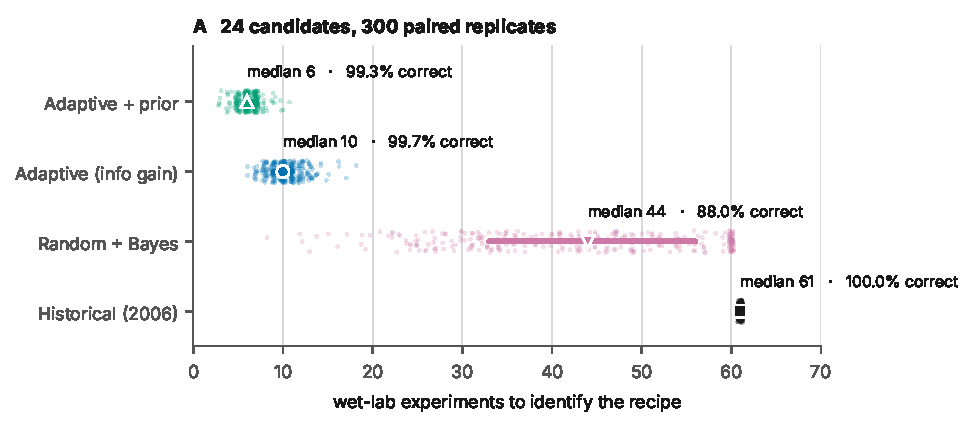
\includegraphics[width=0.84\textwidth]{fig1_main_comparison.pdf}
  \caption{\textbf{Wet-lab cost over 300 paired replicates at $n=24$.} The
  ablation shares the designer's inference exactly and differs only in
  selecting pools at random, which places the saving in experiment selection
  rather than in Bayesian updating.}
  \label{fig:main}
\end{figure}

Over 300 paired replicates the historical protocol spends 61 experiments
every time, by construction. The information-gain designer recovers the
hidden recipe in a
median of 10 (mean 10.3, 99.7\% success), and with a literature prior
up-weighting eight factors in a median of 6 (mean 6.2, 99.3\%). It is cheaper
in 300 of 300 paired runs. The measured median sits at the order the framework
predicts: $O(g^2 d \log n)$ at $g=1$, $d=4$, $n=24$ is about 13.

The load-bearing comparison is the ablation. Identical priors, likelihood and
posterior, with pools drawn at random instead of scored, needs a median of 44
experiments at 88.0\% success (Fig.~\ref{fig:main}). The saving is therefore
attributable to informative experiment selection and not to Bayesian inference
as such --- a distinction that matters because the inference is the expensive
half.

\subsection{An apparent regime boundary, and what it actually was}
\label{sec:scaling}

Yamanaka's 24 candidates were themselves a literature filter, so a method that
works only after such filtering is of limited use. Varying the list from 24 to
60 factors, the designer's wet-lab cost grows as $n^{1.61}$, not
logarithmically. The classical half-removal search shows the opposite pattern:
twice as expensive at $n=24$ (20 against 10 experiments), it grows as $n^{0.36}$
and the curves cross at 48 candidates. Because that algorithm carries no model
of the assay, the crossing localises the deficiency --- not in the inference
and not in the problem, but in proposal generation. Random pools of size 2--12
contain all four essential factors with probability falling as $n^{-4}$.

That was an interpretation of a null result, offered by the authors of the
method it embarrassed, and it deserved a direct test. Holding the scoring rule,
posterior, oracle, recipes, seeds \emph{and} the number of pools scored per
round fixed, and changing only which pools may be scored, the growth exponent
falls from $n^{1.61}$ to $n^{0.43}$ against $n^{0.36}$ for the classical
search. The median at 60 candidates falls from 48 experiments to 15 --- below
the classical algorithm's 27 rather than above it --- at 100\% recovery, where
the classical search has declined to 83\% because the pool-size penalty drags
its positive control toward the noise floor. The saving is zero at 24
candidates (0.6 experiments, $p=0.29$), where the original window already
covered a usable fraction of the space, and grows monotonically: 5.5 at 32, 8.6
at 40, 19.7 at 48 and 34.2 at 60, all paired, all $p < 10^{-3}$.

Two qualifications. The structured generator was written after seeing the
failure it repairs, so it explains that failure rather than predicting it. And
the compute wall is untouched: exact enumeration grows as $n^4$ in hypotheses
and remains the binding constraint past about 60 candidates. What the
experiment establishes is narrower and sufficient --- the regime boundary was
an implementation choice, not a property of information-gain design.

\subsection{Assumed cardinality: a symmetric, silent failure}
\label{sec:cardinality}

\begin{figure}[t]
  \centering
  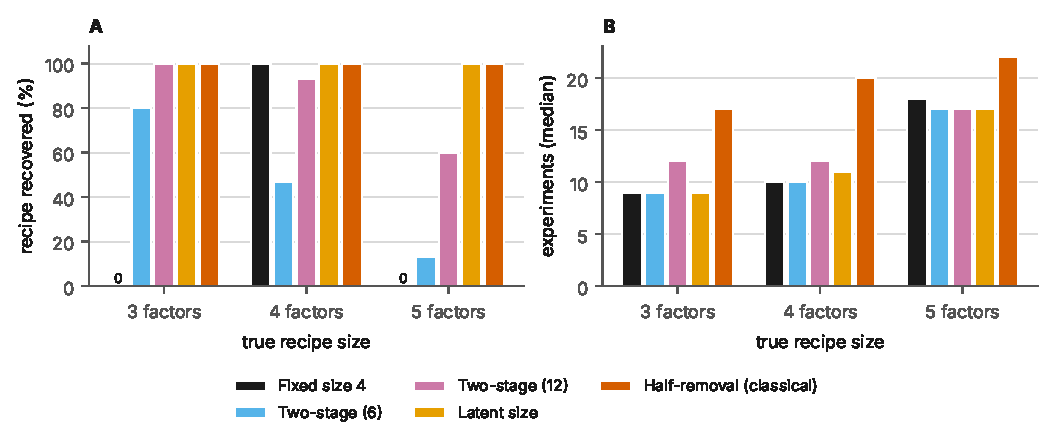
\includegraphics[width=\textwidth]{fig4_cardinality.pdf}
  \caption{\textbf{Recipe size assumed against inferred}, with the oracle
  hiding recipes of three, four and five factors. The fixed designer's failures
  are not hedged: it reports a confidence above 0.99 while returning a recipe
  of the wrong size.}
  \label{fig:cardinality}
\end{figure}

The designer above assumes $k = 4$. With the oracle hiding recipes of three,
four and five factors, a designer fixed at four recovers the exact recipe in
0\% of runs at $k=3$ and 0\% at $k=5$, in both cases reporting a posterior
above 0.99 (Fig.~\ref{fig:cardinality}). The failure is \emph{symmetric}: a
three-factor truth is as fatal as a five-factor one, because the designer finds
the three real factors and appends a spurious fourth. The defect is fixing the
cardinality at all, in either direction.

Making size latent removes it: 100\% recovery at every true size, with the
correct size carrying posterior mass above 0.995, at a premium of 0.9
experiments on the four-factor case it did not need to generalise for
($p = 0.0036$). The classical two-stage remedy --- estimate the count, then
commit --- inherits the failure in proportion to its stage-one budget: with six
experiments it commits to the wrong size in 53\% of $k=4$ runs and 87\% of
$k=5$ runs, recovering 47\% and 13\%. Model-free half-removal, which represents
no size at all, succeeds throughout, which is the cleanest statement of where
the defect lives.

\subsection{The gap assumption against measured data, and the designer run on it}
\label{sec:real}

\begin{figure}[t]
  \centering
  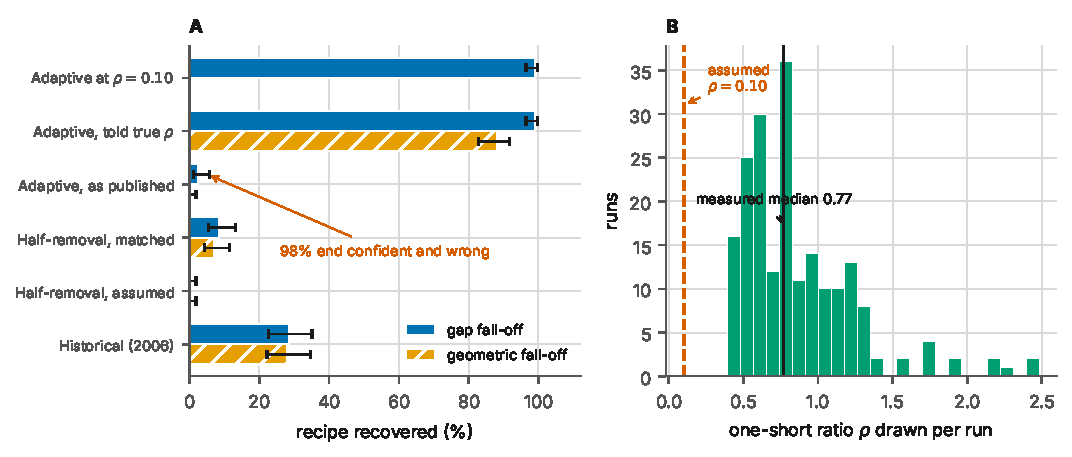
\includegraphics[width=\textwidth]{fig7_measured_gap.pdf}
  \caption{\textbf{Recovery when the gap response is drawn from measurement
  rather than assumed.} (A) 200 paired runs per arm with Wilson intervals,
  under both fall-off shapes. (B) The distribution of $\rho$ drawn per run,
  against the value the oracle assumes.}
  \label{fig:measuredgap}
\end{figure}

Every result above is conditional on gap structure of the assumed depth.
Writing $\delta_p = x_p - x_0$ for a perturbation's pseudobulk profile against
its reference, the empirical analogue of $\rho$ is
$\max_c \lVert\delta_c\rVert / \lVert\delta_{\text{combination}}\rVert$ over
the constituents $c$ of a measured combination. In \citet{norman2019} (K562,
CRISPRa, 131 pairs with both singles measured) the median is \textbf{0.77}
(IQR 0.62--1.03) and \emph{no pair of the 131} falls below 0.20; in the
combinatorial subset of \citet{joung2023} (hESC, 40 TF--TF pairs) the median is
0.77--0.91 under three alternative references, with no pair below 0.20 under
any. Threshold-like functionals lower the Norman median to 0.48 but none
approaches 0.10. The assumed value is five- to eightfold too sharp.

Rather than leave that as a caveat, we ran the method on it: $\rho$ drawn per
replicate from the 131 measured ratios and held fixed across arms, 200 runs per
arm (Fig.~\ref{fig:measuredgap}). Under the gap fall-off the designer as
published recovers the recipe in \textbf{2.5\%} of runs (Wilson 1--6\%) against
99.0\% for the same designer informed of $\rho$ (exact McNemar $p<10^{-4}$).
The failures are not budget exhaustions: no run reached the cap, the median
cost was 9 experiments against 10 for the correctly calibrated reference, and
the mean posterior confidence on runs that ended \emph{wrong} was
\textbf{0.991}.

The classical algorithm is not a fallback. Half-removal recovers 0.0\% with its
assumed threshold and 8.5\% with the threshold rebuilt at the true $\rho$: when
a one-short pool yields 80\% of a complete one, no positivity threshold
separates them, and being told the truth does not help because the information
is not in the readout. The 2006 protocol reaches 28.5\% --- far worse than a
correctly calibrated designer, but with no confidence claim to be wrong about.
Under a geometric fall-off the published designer recovers nothing at all
(0/200) while the matched designer reaches 88.0\%.

\subsection{Inferring the gap response rather than assuming it}
\label{sec:latent}

\begin{figure}[t]
  \centering
  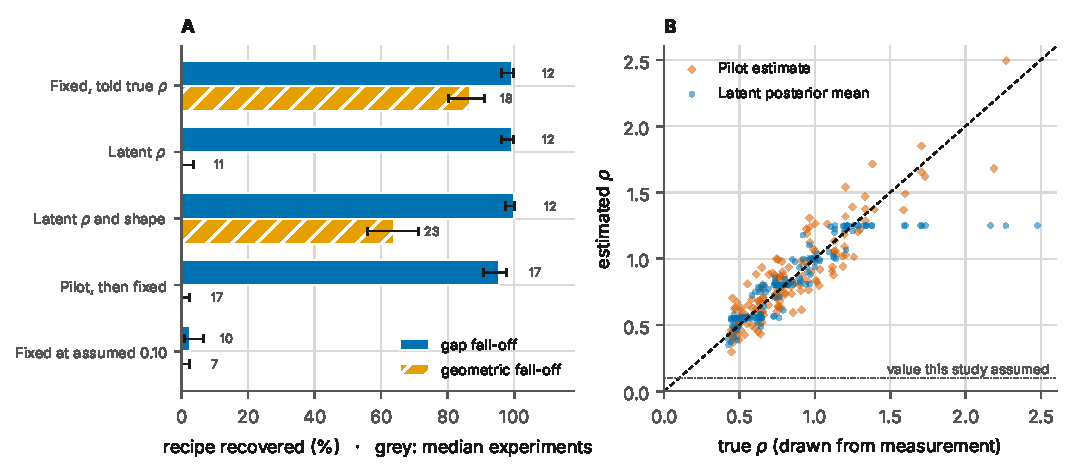
\includegraphics[width=\textwidth]{fig10_latent_gap.pdf}
  \caption{\textbf{Two ways to stop assuming $\rho$.} (A) 150 paired runs per
  arm with Wilson intervals; the grey number beside each bar is that arm's
  median experiment count, since an arm is only cheap if it is also right, and
  the pilot's five calibration tests are counted inside its total. (B)
  Estimated against true $\rho$ under the gap shape, with the identity line;
  the latent estimates flatten at 1.25 because that is the top of the grid.}
  \label{fig:latentgap}
\end{figure}

Section~\ref{sec:real} leaves $\rho$ as something that must be obtained. A
laboratory would calibrate first; the alternative is to carry $\rho$ in the
posterior. Which is cheaper is not obvious: the pilot spends whole experiments
up front and ends in a point estimate with its own Poisson error, while joint
inference spends part of every experiment's evidence on a nuisance parameter.
All arms below use the structured proposals of Section~\ref{sec:scaling}, so
the generator is not a confound.

Under the gap fall-off the answer is unambiguous (Fig.~\ref{fig:latentgap}).
Latent $\rho$ recovers \textbf{99.3\%} at a median of 12 experiments ---
indistinguishable from the oracle arm told the true value (99.3\%, median 12),
at 0.4 experiments on the paired mean. Against the pilot it is both cheaper and
more accurate: 4.7 fewer experiments ($p<10^{-4}$) at 99.3\% against 95.3\%.
Making the shape latent as well costs nothing measurable and recovers 100\%.
The inferred $\rho$ has a median absolute error of 0.06 against a grid spacing
of 0.20--0.25, and a 90\% credible interval over grid cells covers the true
value in 86\% of runs, close to nominal and a little under it, which is the
expected price of a discrete grid.

The geometric fall-off is where the result stops, and how it stops is
informative. Latent $\rho$ with the shape still fixed recovers \textbf{0.7\%}
--- no better than the uncalibrated designer, because the misspecification was
never only in $\rho$. The pilot recovers \textbf{0\%}, and necessarily so: a
pilot measures the one-short step and is structurally blind to what lies beyond
it, so no number it returns can repair a wrong shape. Only the arm treating the
shape as unknown recovers anything, at 64.0\% and a median of 23 experiments
against 86.7\% for an oracle told both. That arm identifies the shape
essentially perfectly --- posterior mass on the true shape above 0.9 in 100\% of
runs --- so what limits it is searching the flat landscape the model describes,
not identifying the model. Under a misspecified shape the $\rho$ interval
covers in 36\% of runs, so the posterior reports the miss rather than
concealing it.

\subsection{Discovery against measured data, with no simulator}
\label{sec:retrospective}

\begin{figure}[t]
  \centering
  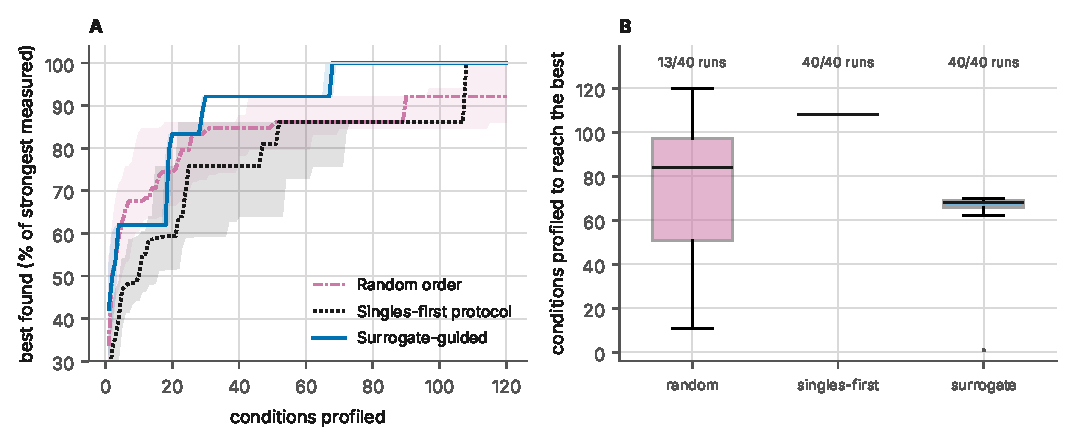
\includegraphics[width=\textwidth]{fig8_retrospective.pdf}
  \caption{\textbf{Sequential discovery where every query returns a
  measurement.} (A) Best condition found so far as a fraction of the strongest
  measured combination, median over 40 replicates with interquartile band. (B)
  Conditions profiled before reaching it; the annotation gives how many
  replicates reached it at all, without which the box is not comparable.}
  \label{fig:retrospective}
\end{figure}

Sections~\ref{sec:real} and~\ref{sec:latent} ground one oracle parameter in
measurement but still query a simulator. The strongest available test removes
it. We built an oracle over \citet{norman2019} that answers only for
conditions the authors actually profiled --- 105 singles, 131 pairs and one
control --- returning the magnitude of the measured pseudobulk shift against
control, perturbed by the dataset's own disagreement across two random halves
of the gene panel (median relative discrepancy 0.049). A condition that was
not profiled raises an error rather than being interpolated, since an
interpolated answer would reinstate the simulation the construction exists to
remove.

That restriction changes the task: with no pools beyond pairs there is nothing
to design, so this is sequential discovery within a measured library rather
than threshold group testing. It tests the half of the claim that survives ---
that choosing the next experiment from a model beats choosing it by protocol.
A surrogate fitting pair response on its constituents' measured singles,
queried by upper-confidence score, reaches the strongest combination in a
median of 68 conditions in 40 of 40 replicates, against 108 for a
singles-first protocol and 84 for random order, which reached it at all in
only 13 of 40. At a budget of 20 conditions the surrogate attains 83\% of the
target against 59\% for the protocol (paired permutation, $p<10^{-4}$;
Fig.~\ref{fig:retrospective}).

The singles-first row should be read as biology before method. A measured
one-short ratio of 0.77 is precisely what makes ``profile the singles, then
the pairs built from the best of them'' nearly sufficient on this landscape.
The simulated assay, in which a single factor yields nothing at all, is the
\emph{easier} of the two problems rather than the harder one --- a point the
simulation-only version of this study could not have reached.

% ===========================================================================
\section{Discussion}

Four conclusions survive the controls, and they are narrower than the headline
saving.

The saving is real but unsurprising once the problem is named. Recognising the
colony assay as stochastic threshold group testing with $g=1$ supplies the
achievable order and the observation that the 2006 protocol operated at
$\Theta(n)$. The contribution is the quantification, with the historical count
as the reference.

The Bayesian apparatus earns its place, but not for the reason we first
reported. Measured against a classical conjunctive search it appeared to lose
beyond 48 candidates; giving it that algorithm's own queries to score removes
the crossing and leaves it at a third of the cost and a higher recovery rate at
every list length tested. The episode is worth stating plainly, because the
first version of this analysis would have been published as a regime claim and
the regime was an artefact. What survives is a compute boundary rather than a
statistical one.

For deployment, the pattern across Sections~\ref{sec:cardinality}
to~\ref{sec:latent} is the paper's most portable finding, and it is the same
finding three times. Recipe size, gap depth, and the fall-off shape beyond the
gap are each a parameter the designer's author must set; each one, set wrongly,
produces not degradation but confident error at a posterior above 0.99; and in
each case the remedy is to make the parameter latent rather than to calibrate
it better. Latent treatment is cheap where it has been measured --- one extra
experiment for size, 0.4 for $\rho$ --- and it supplies the diagnostic a fixed
designer cannot produce even in principle, since a model that assumes four
factors can never doubt the four. Against this, calibrating first is both more
expensive and strictly weaker: a pilot can measure a parameter but cannot
discover that the parameter was the wrong one to measure.

Read together, these results are less a study of one historical screen than a
specification for the evaluator any such search runs inside --- a learned model
of cell state as much as the calibrated oracle used here. Its gap response must
be accurate to within about a factor of two, with under-estimation the safer
error; it must expose uncertainty over structure and not only a score; and its
stopping confidence is trustworthy only to the extent its own model is. The
measured audit adds a fourth requirement and relaxes one assumption: an
evaluator fitted to expression data will present a graded, near-additive
landscape rather than the sharp threshold the 2006 assay suggests, which is
easier to search, but it also means the gap response must be estimated rather
than inherited from a published figure.

\paragraph{Limitations.} The oracle is a simulator calibrated to published
summary figures, and the replay therefore validates the search procedure and
not the oracle; only Section~\ref{sec:real} tests the model against data it was
not built from. Carrying $\rho$ from a transcriptional response magnitude to a
colony rate assumes response magnitude is monotone in assay yield, which pair
data cannot test and on which Sections~\ref{sec:real} and~\ref{sec:latent}
turn. Both measured datasets read out the transcriptome while the 2006 assay
reads out a rare discrete phenotype, so the audit refutes the assumption for
expression-level objectives and constrains, rather than settles, the phenotype
case. The latent treatments are bounded by their grids --- sizes 3--6, $\rho$ at
most 1.25 --- so the fix widens the assumption without eliminating it. And
exact enumeration binds past about 60 candidates, three orders of magnitude
short of the roughly 1,600 human transcription factors.

\paragraph{Appendix and reproducibility.} The supplementary appendix carries
the large campaigns behind the intervals and paired tests (6{,}320 replicates),
the stopping-rule analysis, the classical and two-stage baselines, the
proposal-generator ablation in full, a retrospective benchmark in which every
query returns a measured Norman condition and nothing is simulated, and the
complete statistical report. All code, per-run CSVs and figures are public, and
the statistics layer is tested against closed-form or planted-truth answers.

\paragraph{Acknowledgements.} The experiments, analysis and manuscript were
developed with Claude (Anthropic) as a research tool; all results are
reproducible from the public repository.

\bibliographystyle{unsrtnat}
\bibliography{refs}

\end{document}
